\section{Predictions on $y$}
The difference between this section and the previous is perspective. In $\S$11.6 we focused on the spread of the average of $y$. In other words, $\E*{\widehat y}$.


\nl Wha tif instead, we wanted to focus on the distribution of the values that $y$ can take when $x = x^*$. Recall:
$$y = \underbrace{\beta_0 + \beta_1 x}_{\text{deterministic}} + \underbrace{\varepsilon}_{\text{\say{spread} of } y}$$
and $\Var{y} = \Var{\varepsilon} = \sigma^2$. Our estimator for $y$ at $x^*$ is defined 
$$\widehat y^* = \widehat{\beta_0} + \widehat{\beta_1} x^* + \varepsilon.$$
Since $\varepsilon \sim \operatorname{N}(0,\sigma^2)$.
\begin{align*}
    \E{\widehat{y}^*} &= \E{ \widehat{\beta_0} + \widehat{\beta_1} x^*} + \E{\varepsilon}\\
    &= \E{\widehat{y}(x^*)}\\
    &= \beta_0 + \beta_1 x^*
\end{align*}

Computing variance is surprisingly easy. As before, $\widehat{y}^*$ is a sum of Normal random variables. Hence, $\widehat y^*$ is Normally distributed.

\nl Moreover, our assumption on $\varepsilon$ is that it is independent of $x$.

\nl We have that $S^2$ is independent of $\widehat{\beta_0}$ and $\widehat{\beta_1}$. So 
\begin{align*}
    \Var{\widehat y^*} = \Var{\widehat{\beta_0} + \widehat{\beta_1} x^*} + \Var{\varepsilon} \tag{by independence}\\
    &= \sigma^2 \pars{\dfrac{1}{n} + \dfrac{\pars{x^* - \bar x}^2}{S_xx}} + \sigma^2 \\
    &= \sigma^2 \pars{\red{1} + \over{n} + \dfrac{\pars{x^* - \bar x}^2}{S_xx}}
\end{align*}
\red{This is the only difference from last sections $\Var{\widehat y}$}.

\nl When $\sigma^2$ unknown.
$$\Var{\widehat y^*} = S^2 \pars{1 + \over{n} + \dfrac{\pars{x^* - \bar x}^2}{S_xx}}$$
For the $1 - \alpha$ level confidence interval (two sided)
$$\Pr \pars{ \abs{T} > t_{\alpha/2} (\text{df})} = 1 - \alpha$$
$$\mathcal Z = \dfrac{y^* - \E{\widehat y^*}}{\sigma_{\widehat y^*}}$$
or
$$\mathcal T = \dfrac{y^* - \pars{\widehat{\beta_0} + \widehat{\beta_1} x^*}}{S \displaystyle \sqrt{1 + \over{n} + \dfrac{\pars{x^* - \bar x}^2}{S_xx}}}$$
t-distributed with $n-2$ degrees of freedom and $1-\alpha$ level confidence interval is 
$$\pars{\widehat{\beta_0} + \widehat{\beta_1} x^*} \, \pm \, t_{\alpha/2}(\text{df})S \displaystyle \sqrt{1 + \over{n} + \dfrac{\pars{x^* - \bar x}^2}{S_xx}}$$

\disc Confidence and prediction bands.
\\ In $\S$11.6, we had C.I. for the mean of $\widehat y (x^*)$.
\\ In $\S$11.7, we have C.I. for the spread of $y$ at $x^*$,

\nl In either case, as $x^*$ moves away from $\bar x$, the $\dfrac{(x^* - \bar x)^2}{S_{xx}}$ increases as does the standard error. i.e. the intervals get longer.

%hyperbolic image
\begin{center}
    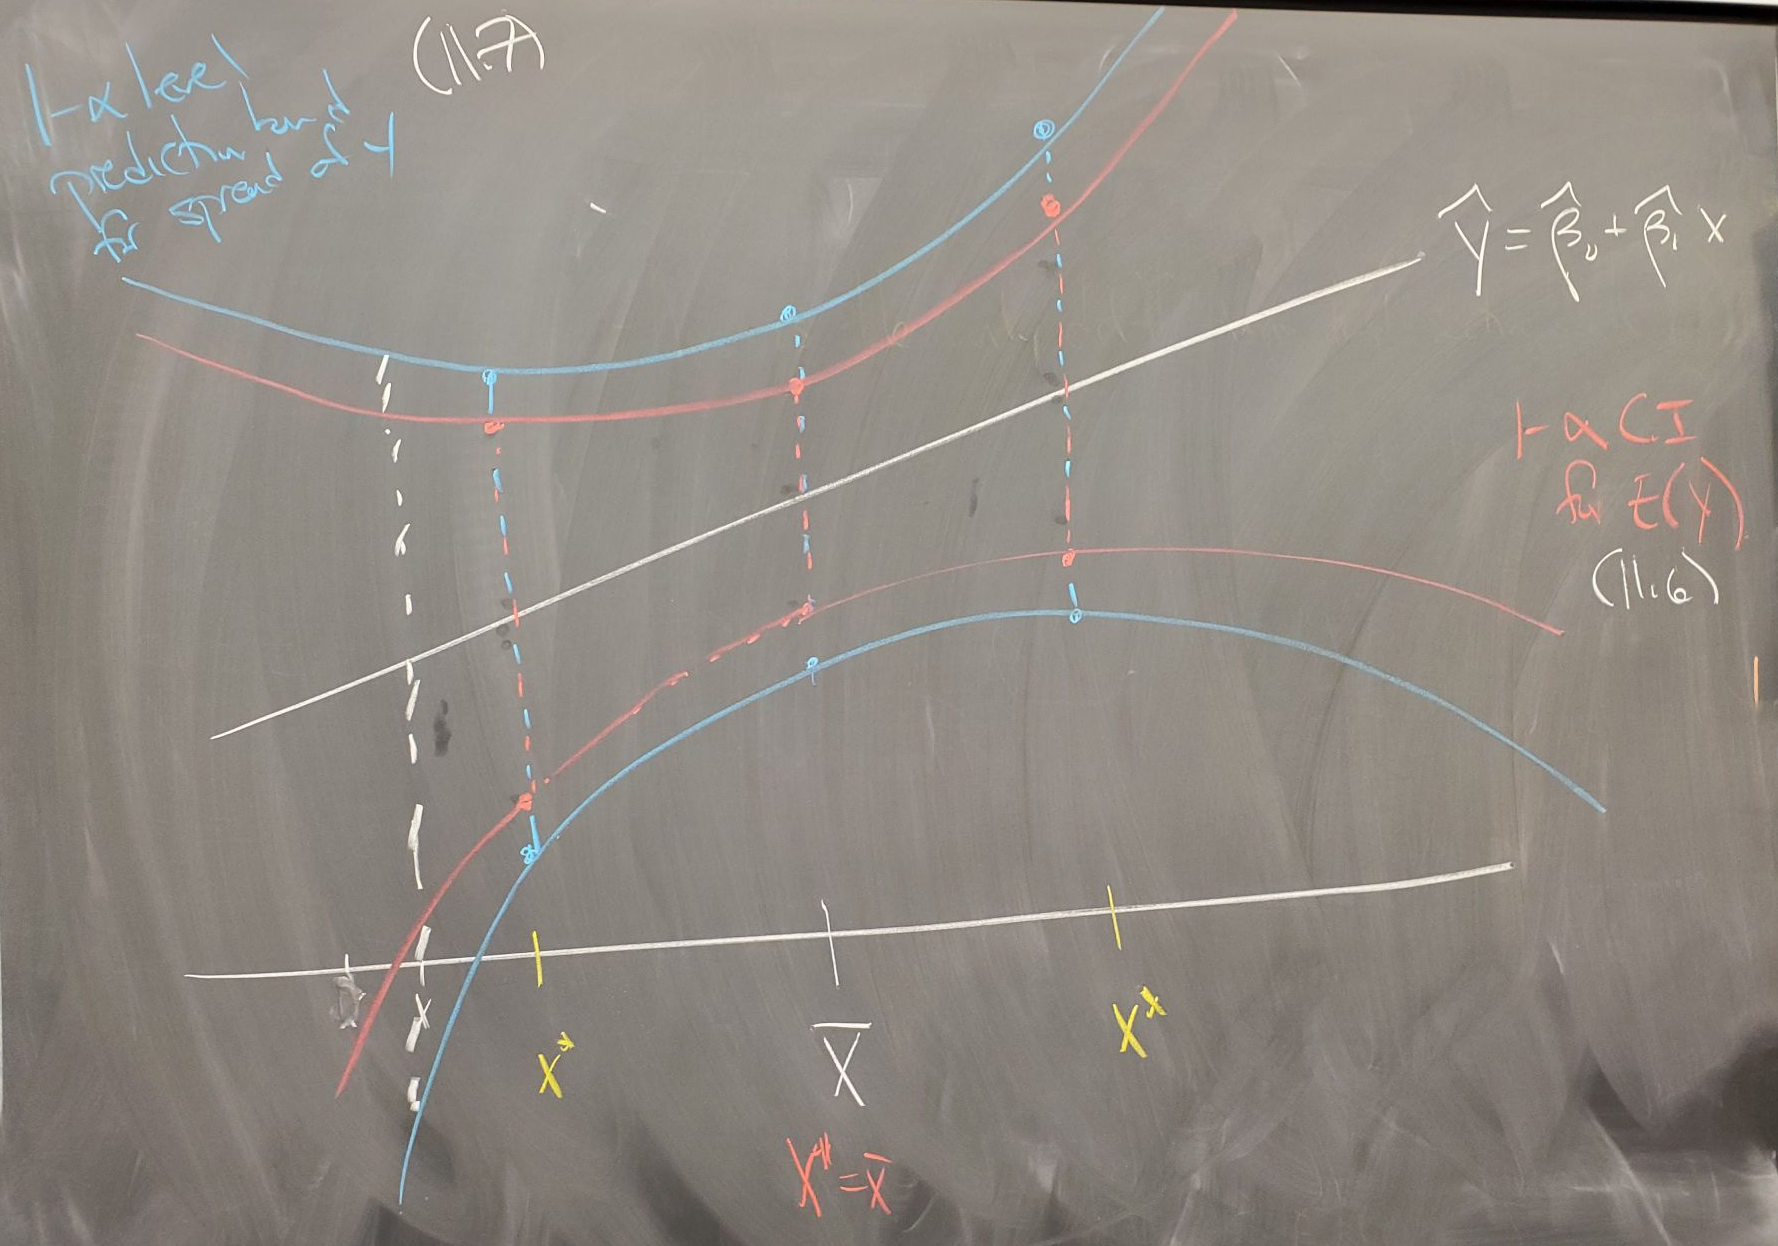
\includegraphics[width=6.5in]{11_7_hyperbola.png}
\end{center}

\noindent \textbf{Example: } Potency of antibiotic when stored at $20^{\circ}$F. Last day we showed that $\E{\widehat y(20)}$ had 90\% confidence interval
$$\setRed \underbrace{\setBlack 39.6 \pm 4.677}_{\text{red cross-section}}$$
What spread of potency would we expect to see with 90\% confidence if stored at $20^{\circ}$F. The same calculation as the last but with new standard error 
$$39.\overline6 \pm 1.812 \sqrt{1 + \over{12} + \frac{1600}{6000}}$$
$$\setBlue \underbrace{\setBlack 39.6 \pm 5.069}_{\text{blue cross-section}}$$


